\chapter{As Propriedades Termodinâmicas e o Estado}
\label{chap:thermodynamicProperties}

    Neste momento de nosso estudo, vamos proceder a um inventário das
    propriedades termodinâmicas que conhecemos até agora. Temos as propriedades
    intensivas próprias, a temperatura \gls{temperature} e a pressão
    \gls{pressure}, as \enquote{intensivadas}: volume específico
    \gls{specificVolume}, energia total específica \gls{intTotalEnergy},
    energia interna específica \gls{intInternalEnergy}, entalpia específica
    \gls{intEnthalpy},  entropia específica \gls{intEntropy}, exergia de fluxo
    \gls{intFlowExergy}, exergia de não-fluxo \gls{intNonFlowExergy} e as
    extensivas --- massa \gls{mass}, volume \gls{volume}, energia total
    \gls{totalEnergy}, energia interna \gls{internalEnergy}, entalpia
    \gls{enthalpy}, entropia \gls{entropy}, exergia de fluxo \gls{flowExergy} e
    exergia de não fluxo \gls{nonFlowExergy}.

    Salientamos, uma vez mais, que as vazões (interações) de massa para dentro
    e para fora de um volume de controle não são em geral propriedades
    termodinâmicas, pois dependem de uma história do processo, muito embora
    tais vazões sejam portadoras das propriedades termodinâmicas. Os valores de
    algumas dessas propriedades podem ser obtidos por meio de instrumentos e
    portanto são mensuráveis, como \gls{mass}, \gls{pressure},
    \gls{temperature}, \gls{volume} e \gls{specificVolume}. Todas as demais
    propriedades são não mensuráveis e os seus valores só podem ser obtidos de
    forma indireta.

    Genericamente por causa do Postulado dos Estados podemos escrever
    $\gls{zAxis} = \gls{zAxis}\functionOf{\gls{xAxis}, \gls{yAxis}}$, onde
    $\gls{xAxis},\gls{yAxis},\gls{zAxis}$ podem ser quaisquer propriedades
    intensivas e $\gls{xAxis},\gls{yAxis}$ devem ser, como já sabemos,
    independentes entre si. Assim, a cada par \gls{xAxis}, \gls{yAxis}
    corresponde um valor de \gls{zAxis}. Observe que estamos usando, por
    conveniência, a notação pela qual confundimos a variável dependente
    \gls{zAxis} com o nome da função
    \gls{zAxis}\functionOf{\gls{xAxis},\gls{yAxis}}. Utilizando-se uma
    representação geométrica na \cref{fig:xyzStateSpace}.

    \begin{figure}[!htb]
        \caption{%
            Representação geométrica do espaço de estados de uma função
            genérica $\gls{zAxis} =
            \gls{zAxis}\functionOf{\gls{xAxis},\gls{yAxis}}$ e o significado de
            suas derivadas parciais.
        }

        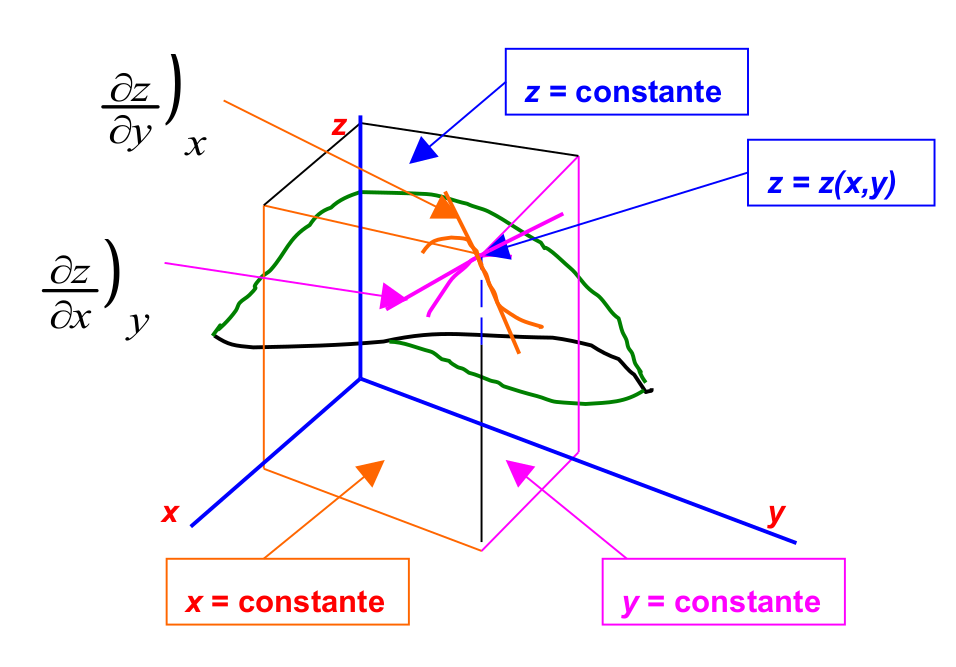
\includegraphics[
            width=\textwidth
        ]   {xyzStateSpace.png}

        \label{fig:xyzStateSpace}
    \end{figure}

    A derivada parcial \ddxconsty{z}{x}{y}, que é uma função
    $M\functionOf{\gls{xAxis},\gls{yAxis}}$, representa nada mais do que a
    tangente à curva produzida pela intersecção da superfície
    \gls{zAxis}\functionOf{\gls{xAxis},\gls{yAxis}} com qualquer plano de
    \gls{yAxis} constante, como mostra a figura. De modo análogo, a derivada
    parcial \ddxconsty{z}{y}{x}, que também é uma função
    $N\functionOf{\gls{xAxis},\gls{yAxis}}$, representa a tangente à curva
    produzida pela intersecção da superfície
    \gls{zAxis}\functionOf{\gls{xAxis},\gls{yAxis}} com qualquer plano de
    \gls{xAxis} constante.  Ressaltamos que, ao contrário do que você poderia
    pensar, \ddxconsty{z}{x}{y} e \ddxconsty{z}{y}{x} são ambas funções tanto de
    \gls{xAxis} como de \gls{yAxis}. Se você fixar essa noção geométrica de
    derivada parcial, provavelmente nunca mais terá problemas para entender e
    utilizar o conceito.


    \section{Um Pouco de Cálculo}

    De $\gls{zAxis} = \gls{zAxis}\functionOf{\gls{xAxis},\gls{yAxis}}$ podemos
    escrever de imediato,
    %
    \begin{equation} \label{eq:5.1}
        \diff{\gls{zAxis}}
        =
        \ddxconsty{
            \gls{zAxis}
        }{
            \gls{xAxis}
        }{
            \gls{yAxis}
        }
        \diff{\gls{xAxis}}
        +
        \ddxconsty{
            \gls{zAxis}
        }{
            \gls{yAxis}
        }{
            \gls{xAxis}
        }
        \diff{\gls{yAxis}}
        =
        M
        \functionOf{
            \gls{xAxis},
            \gls{yAxis}
        }
        \diff{\gls{xAxis}}
        +
        N
        \functionOf{
            \gls{xAxis},
            \gls{yAxis}
        }
        \diff{\gls{yAxis}}\,,
    \end{equation}
    %
    conhecida como a Regra da Cadeia. Além disso, você pode demonstrar que
    (faça!):
    %
    \begin{equation} \label{eq:5.2}
        \ddxconsty{
            \gls{zAxis}
        }{
            \gls{xAxis}
        }{
            \gls{yAxis}
        }
        \functionOf{
            \gls{xAxis},
            \gls{yAxis}
        }
        \ddxconsty{
            x
        }{
            z
        }{
            y
        }
        \functionOf{
            \gls{zAxis},
            \gls{yAxis}
        }
        =
        1
    \end{equation}
    %
    conhecida como a Regra da Inversão. Se você estudar atentamente a
    \cref{eq:5.1}, entenderá as vantagens da notação que adotamos em relação a
    variável dependente e a respectiva função. A primeira derivada refere-se a
    uma função \gls{zAxis}\functionOf{\gls{xAxis},\gls{yAxis}} ao passo que a
    segunda derivada está relacionada a
    \gls{xAxis}\functionOf{\gls{zAxis},\gls{yAxis}}.

    Podemos demonstrar também que, para quaisquer \gls{xAxis}, \gls{yAxis} e
    \gls{zAxis}:
    %
    \begin{equation} \label{eq:5.3}
        \ddxconsty{
            \gls{xAxis}
        }{
            \gls{yAxis}
        }{
            \gls{zAxis}
        }
        \functionOf{
            \gls{yAxis},
            \gls{zAxis}
        }
        \ddxconsty{
            \gls{yAxis}
        }{
            \gls{zAxis}
        }{
            \gls{xAxis}
        }
        \functionOf{
            \gls{xAxis},
            \gls{zAxis}
        }
        \ddxconsty{
            \gls{zAxis}
        }{
            \gls{xAxis}
        }{
            \gls{yAxis}
        }
        \functionOf{
            \gls{xAxis},
            \gls{yAxis}
        }
        -1\,,
    \end{equation}
    %
    conhecida como a Regra Cíclica. Mais ainda,
    %
    \begin{equation} \label{eq:5.4}
        \ddxconsty{
            M
        }{
            \gls{yAxis}
        }{
            \gls{xAxis}
        }
        \functionOf{
            \gls{xAxis},
            \gls{yAxis}
        }
        =
        \ddxconsty{
            N
        }{
            \gls{xAxis}
        }{
            \gls{yAxis}
        }
        \functionOf{
            \gls{xAxis},
            \gls{yAxis}
        }\,,
    \end{equation}
    %
    onde o $M\functionOf{\gls{xAxis},\gls{yAxis}}$ e o
    $N\functionOf{\gls{xAxis},\gls{yAxis}}$ foram definidos anteriormente. Esta
    é a Regra das Derivadas Cruzadas.

    Além disso, podemos expandir as derivadas parciais da seguinte forma:
    %
    \begin{equation}
        \ddxconsty{
            \gls{zAxis}
        }{
            \gls{xAxis}
        }{
            \gls{yAxis}
        }
        =
        \ddxconsty{
            \gls{zAxis}
        }{
            w
        }{
            \gls{yAxis}
        }
        \ddxconsty{
            w
        }{
            \gls{xAxis}
        }{
            \gls{yAxis}
        }\,,
    \end{equation}
    %
    onde $w$ é uma propriedade termodinâmica qualquer distinta de \gls{yAxis}.
    Vamos denominar esta de Regra da Quarta Propriedade.

    Não se assuste, pois este, além do conceito de integral de linha a ser
    discutido, é (quase) todo o cálculo de que precisaremos!


    \section{As Relações de Maxwell}

    Seja a Primeira Lei para sistema fechado,
    %
    \begin{equation} \label{eq:5.5}
        \diff{\gls{intInternalEnergy}}
        =
        \idiff{\gls{specificHeatTransfer}}
        -
        \idiff{\gls{specifcWorkRate}}\,.
    \end{equation}

    Se os processos forem todos reversíveis, então
    %
    \begin{equation} \label{eq:5.6}
        \diff{\gls{intInternalEnergy}}
        =
        \gls{temperature}
        \diff{\gls{intEntropy}}
        -
        \gls{pressure}
        \diff{\gls{specificVolume}}\,.
    \end{equation}

    Esta última equação, conhecida como a \emph{relação fundamental na forma de
    energia interna}, relaciona apenas propriedades e, portanto, pode ser
    integrada por qualquer processo ou caminho que imaginemos, desde que
    respeitemos a relação entre as propriedades ao longo do caminho escolhido.
    Por outro lado, embora nela existam cinco propriedades
    \gls{intInternalEnergy}, \gls{temperature}, \gls{pressure},
    \gls{intEntropy}, \gls{specificVolume}, já sabemos (por que razão?) que
    apenas duas podem ser independentes e as demais serão necessariamente
    dependentes destas duas. Escrevemos então,
    %
    \begin{equation} \label{eq:5.7}
        \diff{\gls{intInternalEnergy}}
        =
        \gls{temperature}
        \functionOf{
            \gls{intEntropy},
            \gls{specificVolume}
        }
        \diff{\gls{intEntropy}}
        -
        \gls{pressure}
        \functionOf{
            \gls{intEntropy},
            \gls{specificVolume}
        }
        \diff{\gls{specificVolume}}\,,
    \end{equation}
    %
    e, pela regra da cadeia, identificamos
    %
    \begin{equation} \label{eq:5.8}
        \gls{temperature}
        \functionOf{
            \gls{intEntropy},
            \gls{specificVolume}
        }
        =
        \ddxconsty{
            \gls{intInternalEnergy}
        }{
            \gls{intEntropy}
        }{
            \gls{specificVolume}
        }
        \functionOf{
            \gls{intEntropy},
            \gls{specificVolume}
        }
        \,\,\,\,\,
        \text{e}
        \,\,\,\,\,
        -\gls{pressure}
        \functionOf{
            \gls{intEntropy},
            \gls{specificVolume}
        }
        =
        \ddxconsty{
            \gls{intInternalEnergy}
        }{
            \gls{specificVolume}
        }{
            \gls{intEntropy}
        }
        \functionOf{
            \gls{intEntropy},
            \gls{specificVolume}
        }\,.
    \end{equation}

    Perceba que poderíamos, então, ter definido rigorosamente a temperatura
    absoluta como a variação da energia interna do sistema fechado com a
    entropia, mantendo-se  constante o volume, ou definido a pressão absoluta,
    como sendo a negação da variação da energia interna com o volume, enquanto
    mantemos a entropia constante.  Dessa maneira  nos livramos do último elo
    da dependência da definição circular para o calor e para o trabalho
    mecânico (lembra-se dessa discussão?).

    Pelas derivadas cruzadas temos
    %
    \begin{equation} \label{eq:5.9}
        \ddxconsty{
            \gls{temperature}
        }{
            \gls{specificVolume}
        }{
            \gls{intEntropy}
        }
        =
        -
        \ddxconsty{
            \gls{pressure}
        }{
            \gls{intEntropy}
        }{
            \gls{specificVolume}
        }\,,
        \tag{\romannumber{1}}
    \end{equation}
    %
    que é uma relação muito interessante para nós, pois envolve três
    propriedades mensuráveis \gls{pressure}, \gls{specificVolume},
    \gls{temperature} e uma não mensurável \gls{intEntropy}.

    Lembra-se da entalpia? Definimos como sendo
    $\gls{intEnthalpy} = \gls{intInternalEnergy} +
    \gls{pressure}\gls{specificVolume}$. Na forma diferencial
    %
    \begin{equation} \label{eq:5.10}
        \diff{\gls{intEnthalpy}}
        =
        \diff{\gls{intInternalEnergy}}
        +
        \gls{pressure}
        \diff{\gls{specificVolume}}
        +
        \gls{specificVolume}
        \diff{\gls{pressure}}\,,
    \end{equation}
    %
    ou, substituindo-se a expressão para \diff{\gls{intInternalEnergy}},
    obtemos a relação fundamental na forma de entalpia:
    %
    \begin{equation} \label{eq:5.11}
        \diff{\gls{intEnthalpy}}
        =
        \gls{temperature}
        \functionOf{
            \gls{intEntropy},
            \gls{pressure}
        }
        \diff{\gls{intEntropy}}
        +
        \gls{specificVolume}
        \functionOf{
            \gls{intEntropy},
            \gls{pressure}
        }
        \diff{\gls{pressure}}\,.
    \end{equation}

    Pela regra da cadeia,
    %
    \begin{equation} \label{eq:5.12}
        \gls{temperature}
        \functionOf{
            \gls{intEntropy},
            \gls{pressure}
        }
        =
        \ddxconsty{
            \gls{intEnthalpy}
        }{
            \gls{intEntropy}
        }{
            \gls{pressure}
        }
        \functionOf{
            \gls{intEntropy},
            \gls{pressure}
        }\,,
    \end{equation}
    %
    \noindent e, também,
    %
    \begin{equation} \label{eq:5.13}
        \gls{specificVolume}
        \functionOf{
            \gls{intEntropy},
            \gls{pressure}
        }
        =
        \ddxconsty{
            \gls{intEnthalpy}
        }{
            \gls{pressure}
        }{
            \gls{intEntropy}
        }
        \functionOf{
            \gls{intEntropy},
            \gls{pressure}
        }\,.
    \end{equation}

    Novamente pela regra das derivadas cruzadas,
    %
    \begin{equation} \label{eq:5.14}
        \ddxconsty{
            \gls{temperature}
        }{
            \gls{pressure}
        }{
            \gls{intEntropy}
        }
        \functionOf{
            \gls{intEntropy},
            \gls{pressure}
        }
        =
        \ddxconsty{
            \gls{specificVolume}
        }{
            \gls{intEntropy}
        }{
            \gls{pressure}
        }
        \functionOf{
            \gls{intEntropy},
            \gls{pressure}
        }\,,
        \tag{\romannumber{2}}
    \end{equation}
    %
    \noindent e mais uma vez obtivemos uma relação de
    \gls{pressure},\gls{specificVolume},\gls{temperature} com \gls{intEntropy}.

    Se (re)definirmos a função (ou energia livre) de Gibbs como sendo
    %
    \begin{equation} \label{eq:5.15}
        \gls{intGibbsFreeEnergy}
        \equiv
        \gls{intEnthalpy}
        -
        \gls{temperature}
        \gls{intEntropy}\,,
    \end{equation}
    %
    \noindent então, na forma diferencial, achamos a relação fundamental na
    forma de função (ou energia livre) de Gibbs:
    %
    \begin{equation} \label{eq:5.16}
        \diff{\gls{intGibbsFreeEnergy}}
        =
        -
        \gls{intEntropy}
        \functionOf{
            \gls{temperature},
            \gls{pressure}
        }
        \diff{\gls{temperature}}
        +
        \gls{specificVolume}
        \functionOf{
            \gls{temperature},
            \gls{pressure}
        }
        \diff{\gls{pressure}}\,,
    \end{equation}
    %
    \noindent de onde extraímos
    %
    \begin{equation} \label{eq:5.17}
        \ddxconsty{
            \gls{specificVolume}
        }{
            \gls{temperature}
        }{
            \gls{pressure}
        }
        \functionOf{
            \gls{temperature},
            \gls{pressure}
        }
        =
        -\ddxconsty{
            \gls{intEntropy}
        }{
            \gls{pressure}
        }{
            \gls{temperature}
        }
        \functionOf{
            \gls{temperature},
            \gls{pressure}
        }\,.
        \tag{\romannumber{3}}
    \end{equation}

    Finalmente, se definirmos a função (ou energia livre) de Helmholtz como
    %
    \begin{equation} \label{eq:5.18}
        \gls{intHelmholtzFreeEnergy}
        \equiv
        \gls{intInternalEnergy}
        -
        \gls{temperature}
        \gls{intEntropy}\,,
    \end{equation}
    %
    \noindent então, na forma diferencial, encontramos a relação fundamental na
    forma de função (ou energia livre) de Helmholtz:
    %
    \begin{equation} \label{eq:5.19}
        \diff{\gls{intHelmholtzFreeEnergy}}
        =
        -\gls{intEntropy}
        \functionOf{
            \gls{temperature},
            \gls{specificVolume}
        }
        \diff{\gls{temperature}}
        -
        \gls{pressure}
        \functionOf{
            \gls{temperature},
            \gls{specificVolume}
        }
        \diff{\gls{specificVolume}}\,,
    \end{equation}
    %
    de onde obtemos a relação,
    %
    \begin{equation} \label{eq:5.20}
        \ddxconsty{
            \gls{pressure}
        }{
            \gls{temperature}
        }{
            \gls{specificVolume}
        }
        \functionOf{
            \gls{temperature},
            \gls{specificVolume}
        }
        =
        \ddxconsty{
            \gls{intEntropy}
        }{
            \gls{specificVolume}
        }{
            \gls{temperature}
        }
        \functionOf{
            \gls{temperature},
            \gls{specificVolume}
        }\,.
        \tag{\romannumber{4}}
    \end{equation}

    Note que as \cref{eq:5.9,eq:5.14,eq:5.17,eq:5.20}
    são as \emph{Relações de Maxwell}, que nos fornecem as combinações de
    \gls{pressure}, \gls{specificVolume}, \gls{temperature} e \gls{intEntropy}
    e que são muito utilizadas para a manipulação das relações termodinâmicas.

    Precisamos ainda definir mais duas propriedades importantes. A primeira é o
    \emph{calor específico a volume constante, \gls{constVolumeSpecificHeat}},
    da forma:
    %
    \begin{equation} \label{eq:5.21}
        \gls{constVolumeSpecificHeat}
        \functionOf{
            \gls{temperature},
            \gls{specificVolume}
        }
        \equiv
        \ddxconsty{
            \gls{intInternalEnergy}
        }{
            \gls{temperature}
        }{
            \gls{specificVolume}
        }
        \functionOf{
            \gls{temperature},
            \gls{specificVolume}
        }\,,
    \end{equation}
    %
    e a outra é o \emph{calor específico a pressão constante
    \gls{constPressureSpecificHeat}}:
    %
    \begin{equation} \label{eq:5.22}
        \gls{constPressureSpecificHeat}
        \functionOf{
            \gls{temperature},
            \gls{pressure}
        }
        =
        \ddxconsty{
            \gls{intEnthalpy}
        }{
            \gls{temperature}
        }{
            \gls{pressure}
        }
        \functionOf{
            \gls{temperature},
            \gls{pressure}
        }\,.
    \end{equation}

    Vamos lembrar uma vez mais que o calor específico a volume constante e a
    pressão constante são propriedades termodinâmicas (intensivas ou
    extensivas?) e, como tal, não estão associados a nenhum processo especial a
    pressão ou volume constante e muito menos têm a ver com o calor
    identificado na fronteira do sistema. Estamos conscientes que chamá-los de
    \enquote{calor específico} é receita para muita confusão, mas estes nomes
    possuem fortes conotações históricas.


    \section{A Equação de Estado}

    Considere apenas a tripla de propriedades intensivas mensuráveis
    \gls{pressure}, \gls{specificVolume}, \gls{temperature}.  Como tudo depende
    da escolha das duas propriedades intensivas independentes, deve estar claro
    que podemos expressar as superfícies tridimensionais de forma:
    $\gls{specificVolume} = \gls{specificVolume}\functionOf{\gls{pressure},
    \gls{temperature}}$, explícita em \gls{specificVolume}, $\gls{pressure} =
    \gls{pressure}\functionOf{\gls{specificVolume}, \gls{temperature}}$,
    explícita em \gls{pressure} e $\gls{temperature} =
    \gls{temperature}\functionOf{\gls{pressure}, \gls{specificVolume}}$,
    explícita em \gls{temperature}, ou, ainda, em quatro dimensões, de forma
    implícita: $f\functionOf{\gls{pressure}, \gls{specificVolume},
    \gls{temperature}} = constante$ (qual seria o valor da constante?).

    A relação entre as propriedades \gls{pressure}, \gls{specificVolume},
    \gls{temperature} é chamada tradicionalmente de \emph{equação de estado
    para a substância pura} em questão. Na análise que se segue, podemos supor,
    por um momento, que já conhecemos as equações de estado ou explícitas em
    \gls{pressure} ou explícitas em \gls{specificVolume}, conforme for
    conveniente.

    Por exemplo, seja conhecida a equação de estado generalizada explícita em
    \gls{specificVolume}:

    \begin{equation}
        \gls{specificVolume}
        =
        \gls{specificVolume}
        \functionOf{
            \gls{pressure},
            \gls{temperature}
        }
        =
        \frac{
            \gls{gasConstant}
            \gls{temperature}
        }{
            \gls{pressure}
        }
        \gls{compressibilityFactor}
        \functionOf{
            \gls{pressure},
            \gls{temperature}
        }\,.
    \end{equation}

    Então, sempre podemos obter a partir de
    $\gls{compressibilityFactor}\functionOf{\gls{pressure}, \gls{temperature}}$
    (faça!):
    %
    \begin{equation}
        \ddxconsty{
            \gls{specificVolume}
        }{
            \gls{temperature}
        }{
            \gls{pressure}
        }
        \functionOf{
            \gls{pressure},
            \gls{temperature}
        }
        =
        \frac{
            \gls{gasConstant}
        }{
            \gls{pressure}
        }
        \left[
            \gls{compressibilityFactor}
            \functionOf{
                \gls{pressure},
                \gls{temperature}
            }
            +
            \gls{temperature}
            \ddxconsty{
                \gls{compressibilityFactor}
            }{
                \gls{temperature}
            }{
                \gls{pressure}
            }
            \functionOf{
                \gls{pressure},
                \gls{temperature}
            }
        \right]
    \end{equation}
    %
    e
    %
    \begin{equation}
        \ddxconsty{
            \gls{specificVolume}
        }{
            \gls{pressure}
        }{
            \gls{temperature}
        }
        \functionOf{
            \gls{pressure},
            \gls{temperature}
        }
        =
        \frac{
            \gls{gasConstant}
            \gls{temperature}
        }{
            \gls{pressure}
        }
        \left[
            \ddxconsty{
                \gls{compressibilityFactor}
            }{
                \gls{pressure}
            }{
                \gls{temperature}
            }
            \functionOf{
                \gls{pressure},
                \gls{temperature}
            }
            -
            \frac{
                \gls{compressibilityFactor}
                \functionOf{
                    \gls{pressure},
                    \gls{temperature}
                }
            }{
                \gls{pressure}
            }
        \right]\,.
    \end{equation}

    Você deve ser capaz de obter expressões análogas em função de
    \gls{temperature}, \gls{specificVolume} para a equação de estado explícita
    em \gls{pressure}.

    \begin{equation}
        \gls{pressure}
        =
        \gls{pressure}
        \functionOf{
            \gls{specificVolume},
            \gls{temperature}
        }
        =
        \frac{
            \gls{gasConstant}
            \gls{temperature}
        }{
            \gls{specificVolume}
        }
        \gls{compressibilityFactor}
        \functionOf{
            \gls{specificVolume},
            \gls{temperature}
        }\,.
    \end{equation}

    Então, podemos obter a partir de
    $\gls{compressibilityFactor}\functionOf{\gls{specificVolume},
    \gls{temperature}}$ (faça!):

    \begin{equation}
        \ddxconsty{
            \gls{pressure}
        }{
            \gls{temperature}
        }{
            \gls{specificVolume}
        }
        \functionOf{
            \gls{specificVolume},
            \gls{temperature}
        }
        =
        \frac{
            \gls{gasConstant}
        }{
            \gls{specificVolume}
        }
        \left[
            \gls{compressibilityFactor}
            \functionOf{
                \gls{specificVolume},
                \gls{temperature}
            }
            +
            \gls{temperature}
            \ddxconsty{
                \gls{compressibilityFactor}
            }{
                \gls{temperature}
            }{
                \gls{specificVolume}
            }
            \functionOf{
                \gls{specificVolume},
                \gls{temperature}
            }
        \right]
    \end{equation}
    %
    \noindent e
    %
    \begin{equation}
        \ddxconsty{
            \gls{pressure}
        }{
            \gls{specificVolume}
        }{
            \gls{temperature}
        }
        \functionOf{
            \gls{specificVolume},
            \gls{temperature}
        }
        =
        \frac{
            \gls{gasConstant}
            \gls{temperature}
        }{
            \gls{specificVolume}
        }
        \left[
            \ddxconsty{
                \gls{compressibilityFactor}
            }{
                \gls{specificVolume}
            }{
                \gls{temperature}
            }
            \functionOf{
                \gls{specificVolume},
                \gls{temperature}
            }
            -
            \frac{
                \gls{compressibilityFactor}
                \functionOf{
                    \gls{specificVolume},
                    \gls{temperature}
                }
            }{
                \gls{specificVolume}
            }
        \right]\,.
    \end{equation}


    \section{A Energia Interna a Partir da Temperatura e do Volume}

    Vamos supor que a temperatura \gls{temperature} e o volume específico
    \gls{specificVolume} de uma determinada substância pura sejam escolhidos
    como propriedades independentes. Então todas as demais propriedades são
    dependentes de \gls{temperature}, \gls{specificVolume}. A pressão
    \gls{pressure} pode ser expressa como $\gls{pressure} =
    \gls{pressure}\functionOf{\gls{temperature}, \gls{specificVolume}}$ e a
    equação de estado é explícita em \gls{pressure}. Deve ter ficado claro para
    você que também conhecemos as propriedades termodinâmicas
    $\ddxconsty{\gls{pressure}}{\gls{temperature}}{\gls{specificVolume}}
    \functionOf{\gls{temperature},\gls{specificVolume}}$ e também $
    \ddxconsty{\gls{pressure}}{\gls{specificVolume}}{\gls{temperature}}
    \functionOf{\gls{temperature},\gls{specificVolume}}$ mesmo que estas tenham
    que ser determinados numericamente. Então a energia interna será
    %
    \begin{equation} \label{eq:5.23}
        \gls{intInternalEnergy}
        =
        \gls{intInternalEnergy}
        \functionOf{
            \gls{temperature},
            \gls{specificVolume}
        }\,,
    \end{equation}
    %
    e pela regra da cadeia,
    %
    \begin{equation} \label{eq:5.24}
        \diff{\gls{intInternalEnergy}}=
        \ddxconsty{
            \gls{intInternalEnergy}
        }{
            \gls{temperature}
        }{
            \gls{specificVolume}
        }
        \functionOf{
            \gls{temperature},
            \gls{specificVolume}
        }
        \diff{\gls{temperature}}+
        \ddxconsty{
            \gls{intInternalEnergy}
        }{
            \gls{specificVolume}
        }{
            \gls{temperature}
        }
        \functionOf{
            \gls{temperature},
            \gls{specificVolume}
        }
        \diff{\gls{specificVolume}}
    \end{equation}
    %
    mas
    %
    \begin{equation} \label{eq:5.25}
        \ddxconsty{
            \gls{intInternalEnergy}
        }{
            \gls{temperature}
        }{
            \gls{specificVolume}
        }
        =
        \gls{constVolumeSpecificHeat}
        \functionOf{
            \gls{temperature},
            \gls{specificVolume}
        }\,,
    \end{equation}
    %
    e, pela relação fundamental na forna de energia interna:
    %
    \begin{equation} \label{eq:5.26}
        \ddxconsty{
            \gls{intInternalEnergy}
        }{
            \gls{specificVolume}
        }{
            \gls{temperature}
        }
        \functionOf{
            \gls{temperature},
            \gls{specificVolume}
        }
        =
        \gls{temperature}
        \ddxconsty{
            \gls{intEntropy}
        }{
            \gls{specificVolume}
        }{
            \gls{temperature}
        }
        \functionOf{
            \gls{temperature},
            \gls{specificVolume}
        }
        -
        \gls{pressure}
        \functionOf{
            \gls{temperature},
            \gls{specificVolume}
        }\,.
    \end{equation}

    Finalmente, substituindo-se
    $\ddxconsty{\gls{intEntropy}}{\gls{specificVolume}}{\gls{temperature}}$ por
    $\ddxconsty{\gls{pressure}}{\gls{temperature}}{\gls{specificVolume}}$
    devido à Relação de Maxwell \ref{eq:5.17}:

    \begin{equation} \label{eq:5.27}
        \diff{\gls{intInternalEnergy}}
        =
        \gls{constVolumeSpecificHeat}
        \functionOf{
            \gls{temperature},
            \gls{specificVolume}
        }
        \diff{\gls{temperature}}
        +
        \left[
            \gls{temperature}
            \ddxconsty{
            \gls{pressure}
        }{
            \gls{temperature}
        }{
            \gls{specificVolume}
        }
            \functionOf{
                \gls{temperature},
                \gls{specificVolume}
            }
            -
            \gls{pressure}
            \functionOf{
                \gls{temperature},
                \gls{specificVolume}
            }
        \right]
        \diff{\gls{specificVolume}}\,,
    \end{equation}
    %
    na qual a relação funcional de \gls{temperature},\gls{specificVolume} foi
    enfatizada. Ao integrarmos esta expressão entre dois estados dados por
    $(\state{\gls{temperature}}{1},\state{\gls{specificVolume}}{1})$ e
    $(\state{\gls{temperature}}{2},\state{\gls{specificVolume}}{2})$ obtemos:
    %
    \begin{equation} \label{eq:5.28}
        \begin{aligned}
        \gls{intInternalEnergy}
        \functionOf{
            \state{\gls{temperature}}{2},
            \state{\gls{specificVolume}}{2}
        }
        -
        \gls{intInternalEnergy}
        \functionOf{
            \state{\gls{temperature}}{1},
            \state{\gls{specificVolume}}{1}
        }
        &=
        \int\limits^{
            \state{\gls{intInternalEnergy}}{2}
        }_{
            \state{\gls{intInternalEnergy}}{1}
        }{
            \diff{\gls{intInternalEnergy}}
        }\\
        &=
        \int\limits^{
            \state{\gls{temperature}}{2}
        }_{
            \state{\gls{temperature}}{1}
        }{
            \gls{constVolumeSpecificHeat}
            \functionOf{
                \gls{temperature},
                \gls{specificVolume}
            }
        }\diff{\gls{temperature}}
        +
        \int\limits^{\state{\gls{specificVolume}}{2}}_{\state{\gls{specificVolume}}{1}}{
            \left[
                \gls{temperature}
                \ddxconsty{
                    \gls{pressure}
                }{
                    \gls{temperature}
                }{
                    \gls{specificVolume}
                }
                \functionOf{
                    \gls{temperature},
                    \gls{specificVolume}
                }
                -
                \gls{pressure}
                \functionOf{
                    \gls{temperature},
                    \gls{specificVolume}
                }
            \right]
        }\diff{\gls{specificVolume}}\\\,.
        \end{aligned}
    \end{equation}

    O resultado do lado esquerdo da \cref{eq:5.28} será simplesmente
    $\state{\gls{intInternalEnergy}}{2}\functionOf{\state{\gls{temperature}}{2},
    \state{\gls{specificVolume}}{2}} -
    \state{\gls{intInternalEnergy}}{1}\functionOf{\state{\gls{temperature}}{1},
    \state{\gls{specificVolume}}{1}}$, o que era de se esperar, pois as
    propriedades termodinâmicas, como vimos, sempre têm uma base arbitrária. A
    variação da propriedade, por sua vez, não pode e nem deve depender de base
    alguma, pois seria um contra-senso e um absurdo se os resultados físicos de
    calor e trabalho resultantes da Primeira Lei estivessem vinculados a uma
    base especificada da energia interna!

    Agora do lado direito da \cref{eq:5.28} vemos que para que a primeira
    parcela da direita possa ser integrada em \gls{temperature}, deverá ser
    fornecida uma relação entre o volume \gls{specificVolume} e
    \gls{temperature}. Para que a segunda parcela à direita possa ser integrada
    em \gls{specificVolume}, deverá ser fornecida uma relação entre a
    temperatura \gls{temperature} e \gls{specificVolume}. Note que os valores
    de cada uma dessas integrais individuais dependem das relações escolhidas.
    De fato, estamos diante de exemplos de integrais de linha, que é a última
    peça do Cálculo que nos faltava.

    Note também, que a determinação de $\state{\gls{intInternalEnergy}}{2} -
    \state{\gls{intInternalEnergy}}{1}$ não deve depender de processo ou
    caminho de integração, ou seja, embora cada uma das integrais à direita da
    \cref{eq:5.28} dependa das relações arbitrárias entre \gls{temperature} e
    \gls{specificVolume}, a resultante da soma conjunta das integrais deve ser
    independente de quaisquer caminhos de integração escolhidos. De todos os
    possíveis caminhos de integração, logo percebemos que alguns caminhos de
    integração são mais convenientes que outros. A primeira parcela poderá
    corresponder a uma isovolumétrica, pois ao longo dos caminhos de integração
    em que o volume \gls{specificVolume} permanece constante, a outra parcela
    se anula. Do outro lado, a segunda parcela poderá ser uma isotérmica, pois
    ao longo dos caminhos de integração em que a temperatura \gls{temperature}
    é constante, é a primeira parcela que, por sua vez, desaparece. Em razão
    disso, concluímos que para a determinação da variação da energia interna
    \gls{intInternalEnergy} em função de \gls{temperature} e
    \gls{specificVolume}, o melhor caminho de integração será aquele composto
    de isovolumétricas e isotérmicas. Deve ficar claro para você que o número
    de isotérmicas e isovolumétricas é arbitrário, da mesma forma que se você
    puder andar apenas em ângulos retos para ir de um lugar a outro, ainda
    assim poderá fazê-lo ao longo de infinitas possibilidades...

    Para que você tenha uma visão mais concreta, seja uma equação de estado
    explícita em \gls{pressure}, por exemplo a equação de Van der Waals, que já
    conhecemos:
    %
    \begin{equation*}
        \gls{pressure}
        \functionOf{
            \gls{temperature},
            \gls{specificVolume}
        }
        =
        \frac{
            \gls{gasConstant}
            \gls{temperature}
        }{
            \gls{specificVolume}
            -
            b
        }
        -
        \frac{
            a
        }{
            \gls{specificVolume}^2
        }\,,
    \end{equation*}
    %
    donde obtemos
    %
    \begin{equation} \label{eq:5.29}
        \ddxconsty{
            \gls{pressure}
        }{
            \gls{temperature}
        }{
            \gls{specificVolume}
        }
        =
        \frac{
            \gls{gasConstant}
        }{
            \gls{specificVolume}
            -
            b
        }\,,
    \end{equation}
    %
    e então as isotermas da energia interna são da forma,
    %
    \begin{equation} \label{eq:5.30}
        \diff{\gls{intInternalEnergy}}_{\gls{temperature}}
        =
        \left[
            \gls{temperature}
            \ddxconsty{
                \gls{pressure}
            }{
                \gls{temperature}
            }{
                \gls{specificVolume}
            }
            -
            \gls{pressure}
        \right]
        \diff{\gls{specificVolume}}_{\gls{temperature}}
        =
        \left(
            \frac{
                \gls{gasConstant}
                \gls{temperature}
            }{
                \gls{specificVolume}
                -
                b
            }
            -
            \gls{pressure}
        \right)
        \diff{\gls{specificVolume}}_{\gls{temperature}}
        =
        \frac{
            a
        }{
            \gls{specificVolume}^2
        }
        \diff{\gls{specificVolume}}_T\,,
    \end{equation}
    %
    expressão que integrada, fornece, ao longo de qualquer isoterma
    \gls{temperature}, desde o volume \state{\gls{specificVolume}}{1} até o
    volume \state{\gls{specificVolume}}{2}, isto é, integrando-se de
    $(\gls{temperature}, \state{\gls{specificVolume}}{1})$ até
    $(\gls{temperature}, \state{\gls{specificVolume}}{2})$:
    %
    \begin{equation} \label{eq:5.31}
        \left(
            \state{\gls{intInternalEnergy}}{2}
            -
            \state{\gls{intInternalEnergy}}{1}
        \right)_{\gls{temperature}}
        =
        a
        \left(
            \frac{1}{\state{\gls{specificVolume}}{1}}
            -
            \frac{1}{\state{\gls{specificVolume}}{2}}
        \right)\,.
    \end{equation}

    Note, por outro lado, que para determinarmos as integrais isovolumétricas,
    precisamos conhecer o comportamento do calor específico a volume constante
    $\gls{constVolumeSpecificHeat}\functionOf{\gls{temperature},
    \gls{specificVolume}}$, o que não é nada conveniente. Como resolver isso? A
    solução completa do problema, como veremos, depende do que já estudamos
    sobre as propriedades de uma substância pura, em particular na região de
    gás perfeito.

    Veja o esquema na \cref{fig:integrationLinesTv}, no qual estão
    representados no plano \gls{temperature}-\gls{specificVolume} pelo menos
    dois caminhos de integração: 1-3-2 e 1-4-5-2.

    \begin{figure}[!htb]
        \caption{%
            Caminhos de integração no plano
            \gls{temperature}-\gls{specificVolume}.
        }

        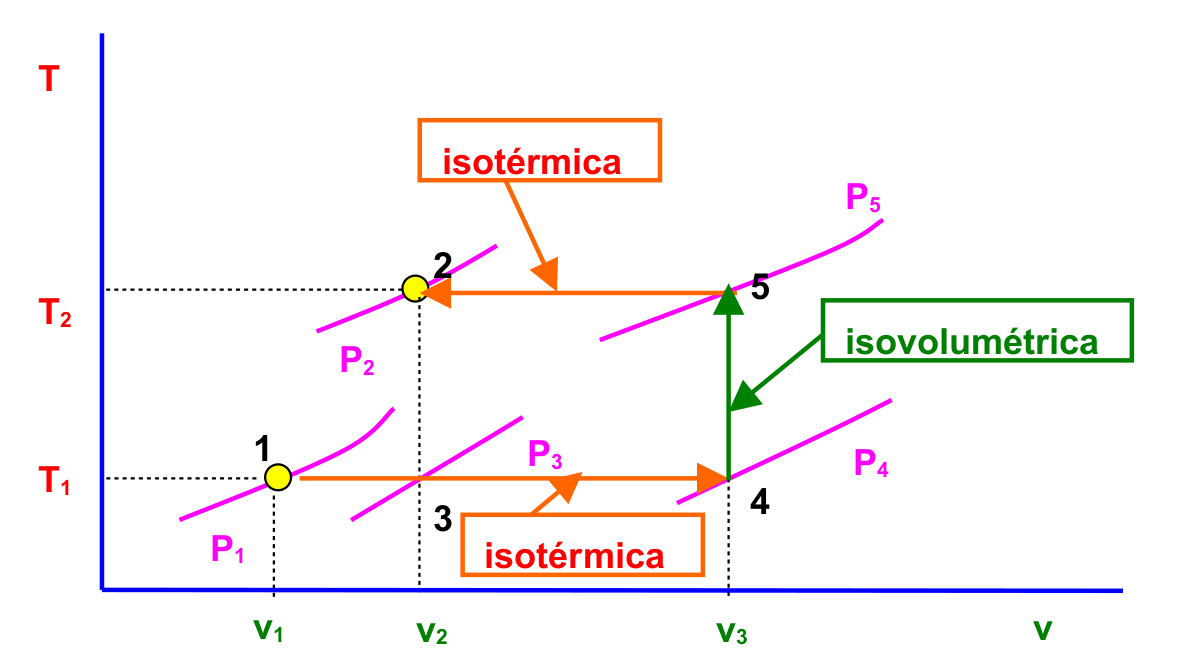
\includegraphics[
            width=0.75\textwidth
        ]   {integrationLinesTv.png}

        \label{fig:integrationLinesTv}
    \end{figure}

    As pressões correspondentes ao segundo caminho são muito menores do que no
    caminho 1-3-2. Em compensação, existe uma isotérmica a mais!

    Integrando-se ao longo do caminho 1-3-2:
    %
    \begin{equation} \label{eq:5.32}
        \begin{aligned}
            \state{\gls{intInternalEnergy}}{2}
            \functionOf{
                \state{\gls{temperature}}{2},
                \state{\gls{specificVolume}}{2}
            }
            -
            \state{\gls{intInternalEnergy}}{1}
            \functionOf{
                \state{\gls{temperature}}{1},
                \state{\gls{specificVolume}}{1}
            }
            &=
            \left[
                \state{\gls{intInternalEnergy}}{2}
                \functionOf{
                    \state{\gls{temperature}}{2},
                    \state{\gls{specificVolume}}{2}
                }
                -
                \state{\gls{intInternalEnergy}}{3}
                \functionOf{
                    \state{\gls{temperature}}{1},
                    \state{\gls{specificVolume}}{2}
                }
            \right]_{\state{\gls{specificVolume}}{2}}\\
            &+
            \left[
                \state{\gls{intInternalEnergy}}{3}
                \functionOf{
                    \state{\gls{temperature}}{1},
                    \state{\gls{specificVolume}}{2}
                }
                -
                \state{\gls{intInternalEnergy}}{1}
                \functionOf{
                    \state{\gls{temperature}}{1},
                    \state{\gls{specificVolume}}{1}
                }
            \right]_{\state{\gls{temperature}}{1}}\,,
        \end{aligned}
    \end{equation}
    %
    ou seja, uma isovolumétrica em \state{\gls{specificVolume}}{2} seguida de
    uma isotérmica em \state{\gls{temperature}}{1}. Substituindo-se a
    isovolumétrica:
    %
    \begin{equation} \label{eq:5.33}
        \begin{aligned}
        \state{\gls{intInternalEnergy}}{2}
        \functionOf{
            \state{\gls{temperature}}{2},
            \state{\gls{specificVolume}}{2}
        }
        -
        \state{\gls{intInternalEnergy}}{1}
        \functionOf{
            \state{\gls{temperature}}{1},
            \state{\gls{specificVolume}}{1}
        }
        &=
        \int\limits_{
            \state{\gls{temperature}}{1}
        }^{
            \state{\gls{temperature}}{2}
        }{
            \gls{constVolumeSpecificHeat}
            \functionOf{
                \gls{temperature},
                \state{\gls{specificVolume}}{2}
            }
        }\diff{\gls{temperature}}\\
        &+
        \left[
            \state{\gls{intInternalEnergy}}{3}
            \functionOf{
                \state{\gls{temperature}}{1},
                \state{\gls{specificVolume}}{2}
            }
            -
            \state{\gls{intInternalEnergy}}{1}
            \functionOf{
                \state{\gls{temperature}}{1},
                \state{\gls{specificVolume}}{1}
            }
        \right]_{\state{\gls{temperature}}{1}}\,,
        \end{aligned}
    \end{equation}

    No caso exemplo da equação de estado de Van der Waals, resulta:
    %
    \begin{equation} \label{eq:5.34}
        \state{\gls{intInternalEnergy}}{2}
        \functionOf{
            \state{\gls{temperature}}{2},
            \state{\gls{specificVolume}}{2}
        }
        -
        \state{\gls{intInternalEnergy}}{1}
        \functionOf{
            \state{\gls{temperature}}{1},
            \state{\gls{specificVolume}}{1}
        }
        =
        \int\limits_{
            \state{\gls{temperature}}{1}
        }^{
            \state{\gls{temperature}}{2}
        }{
            \gls{constVolumeSpecificHeat}
            \functionOf{
                \gls{temperature},
                \state{\gls{specificVolume}}{2}
            }
        }\diff{\gls{temperature}}
        +
        a
        \left[
            \frac{1}{\state{\gls{specificVolume}}{1}}
            -
            \frac{1}{\state{\gls{specificVolume}}{2}}
        \right]\,.
    \end{equation}

    Por outro lado, integrando-se ao longo do caminho 1-4-5-2:
    %
    \begin{equation} \label{eq:5.35}
    \begin{aligned}
        \state{\gls{intInternalEnergy}}{2}
        \functionOf{
            \state{\gls{temperature}}{2},
            \state{\gls{specificVolume}}{2}
        }
        -
        \state{\gls{intInternalEnergy}}{1}
        \functionOf{
            \state{\gls{temperature}}{1},
            \state{\gls{specificVolume}}{1}
        }
        &=
        \left[
            \state{\gls{intInternalEnergy}}{2}
            \functionOf{
                \state{\gls{temperature}}{2},
                \state{\gls{specificVolume}}{2}
            }
            -
            \state{\gls{intInternalEnergy}}{5}
            \functionOf{
                \state{\gls{temperature}}{2},
                \state{\gls{specificVolume}}{3}
            }
        \right]_{\state{\gls{temperature}}{2}}\\
        &+
        \left[
            \state{\gls{intInternalEnergy}}{5}
            \functionOf{
                \state{\gls{temperature}}{2},
                \state{\gls{specificVolume}}{3}
            }
            -
            \state{\gls{intInternalEnergy}}{4}
            \functionOf{
                \state{\gls{temperature}}{1},
                \state{\gls{specificVolume}}{3}
            }
        \right]_{\state{\gls{specificVolume}}{5}}\\
        &+
        \left[
            \state{\gls{intInternalEnergy}}{4}
            \functionOf{
                \state{\gls{temperature}}{1},
                \state{\gls{specificVolume}}{3}
            }
            -
            \state{\gls{intInternalEnergy}}{1}
            \functionOf{
                \state{\gls{temperature}}{1},
                \state{\gls{specificVolume}}{1}
            }
        \right]_{\state{\gls{temperature}}{1}}\,,
    \end{aligned}
    \end{equation}
    %
    ou seja, uma isotérmica em \state{\gls{temperature}}{2} , seguida de uma
    isovolumétrica em \state{\gls{specificVolume}}{3}, seguida de uma isotérmica
    em \state{\gls{temperature}}{1}. Substituindo-se a isovolumétrica:
    %
    \begin{equation} \label{eq:5.36}
    \begin{aligned}
        \state{\gls{intInternalEnergy}}{2}
        \functionOf{
            \state{\gls{temperature}}{2},
            \state{\gls{specificVolume}}{2}
        }
        -
        \state{\gls{intInternalEnergy}}{1}
        \functionOf{
            \state{\gls{temperature}}{1},
            \state{\gls{specificVolume}}{1}
        }
        &=
        \left[
            \state{\gls{intInternalEnergy}}{2}
            \functionOf{
                \state{\gls{temperature}}{2},
                \state{\gls{specificVolume}}{2}
            }
            -
            \state{\gls{intInternalEnergy}}{5}
            \functionOf{
                \state{\gls{temperature}}{2},
                \state{\gls{specificVolume}}{3}
            }
        \right]_{\state{\gls{temperature}}{2}}\\
        &+
        \int\limits_{
            \state{\gls{temperature}}{1}
        }^{
            \state{\gls{temperature}}{2}
        }{
            \gls{constVolumeSpecificHeat}
            \functionOf{
                \gls{temperature},
                \state{\gls{specificVolume}}{5}
            }
        }\diff{\gls{temperature}}\\
        &+
        \left[
            \state{\gls{intInternalEnergy}}{4}
            \functionOf{
                \state{\gls{temperature}}{1},
                \state{\gls{specificVolume}}{3}
            }
            -
            \state{\gls{intInternalEnergy}}{1}
            \functionOf{
                \state{\gls{temperature}}{1},
                \state{\gls{specificVolume}}{1}
            }
        \right]_{\state{\gls{temperature}}{1}}\,,
    \end{aligned}
    \end{equation}

    No caso exemplo da equação de estado de Van der Waals, resulta:

    \begin{equation} \label{eq:5.37}
        \state{\gls{intInternalEnergy}}{2}
        -
        \state{\gls{intInternalEnergy}}{1}
        =
        a
        \left[
            \frac{1}{\state{\gls{specificVolume}}{5}}
            -
            \frac{1}{\state{\gls{specificVolume}}{2}}
        \right]
        +
        \int\limits_{
            \state{\gls{temperature}}{1}
        }^{
            \state{\gls{temperature}}{2}
        }{
            \gls{constVolumeSpecificHeat}
            \functionOf{
                \gls{temperature},
                \state{\gls{specificVolume}}{5}
            }
        }\diff{\gls{temperature}}\\
        +
        a
        \left[
            \frac{1}{\state{\gls{specificVolume}}{1}}
            -
            \frac{1}{\state{\gls{specificVolume}}{5}}
        \right]\,.
    \end{equation}

    Embora a determinação de $\state{\gls{intInternalEnergy}}{2} -
    \state{\gls{intInternalEnergy}}{1}$ pareça resolvida, restam ainda em
    qualquer um dos casos as avaliações das integrais isovolumétricas de
    $\gls{constVolumeSpecificHeat}\functionOf{\gls{temperature},
    \gls{specificVolume}}$. Antes de desenvolvermos uma possível solução para
    isso, vamos apresentar a expressão para a variação da entropia em função de
    \gls{temperature},\gls{specificVolume}.


    \section{A Entropia a Partir da Temperatura e do Volume}

    A partir da relação fundamental na forma de energia interna \cref{eq:5.7}:
    %
    \begin{equation} \label{eq:5.38}
        \ddxconsty{
            \gls{intInternalEnergy}
        }{
            \gls{temperature}
        }{
            \gls{specificVolume}
        }
        \functionOf{
            \gls{temperature},
            \gls{specificVolume}
        }
        =
        \gls{temperature}
        \ddxconsty{
            \gls{intEntropy}
        }{
            \gls{temperature}
        }{
            \gls{specificVolume}
        }
        \functionOf{
            \gls{temperature},
            \gls{specificVolume}
        }
        =
        \gls{constVolumeSpecificHeat}
        \functionOf{
            \gls{temperature},
            \gls{specificVolume}
        }\,.
    \end{equation}

    Escrevendo $\gls{intEntropy}=
    \gls{intEntropy}\functionOf{\gls{temperature},\gls{specificVolume}}$ pela
    regra da cadeia, expandimos para:
    %
    \begin{equation} \label{eq:5.39}
        \diff{\gls{intEntropy}}
        =
        \ddxconsty{
            \gls{intEntropy}
        }{
            \gls{temperature}
        }{
            \gls{specificVolume}
        }
        \functionOf{
            \gls{temperature},
            \gls{specificVolume}
        }
        \diff{\gls{temperature}}
        +
        \ddxconsty{
            \gls{intEntropy}
        }{
            \gls{specificVolume}
        }{
            \gls{temperature}
        }
        \functionOf{
            \gls{temperature},
            \gls{specificVolume}
        }
        \diff{\gls{specificVolume}}\,,
    \end{equation}
    %
    e, portanto,
    %
    \begin{equation} \label{eq:5.40}
        \diff{\gls{intEntropy}}
        =
        \gls{constVolumeSpecificHeat}
        \functionOf{
            \gls{temperature},
            \gls{specificVolume}
        }
        \frac{
            \diff{\gls{temperature}}
        }{
            \gls{temperature}
        }
        +
        \ddxconsty{
            \gls{pressure}
        }{
            \gls{temperature}
        }{
            \gls{specificVolume}
        }
        \functionOf{
            \gls{temperature},
            \gls{specificVolume}
        }
        \diff{\gls{specificVolume}}\,.
    \end{equation}


    \section{%
        A Entalpia e a Entropia a Partir da Temperatura e da Pressão
    }

    Consideremos agora \gls{temperature},\gls{pressure} como variáveis
    independentes. Por razões de conveniência computacional, \gls{temperature}
    e \gls{pressure}, assim como \gls{temperature},\gls{vaporQuality} ou
    \gls{pressure},\gls{vaporQuality}, na saturação, serão denominadas
    variáveis primárias. Portanto, $\gls{specificVolume} =
    \gls{specificVolume}\functionOf{\gls{pressure}, \gls{temperature}}$ é a
    equação de estado explícita em \gls{specificVolume}. Como antes, a partir
    de $\gls{intEnthalpy} = \gls{intEnthalpy}\functionOf{\gls{temperature},
    \gls{pressure}}$, pela regra da cadeia, expandimos para:
    %
    \begin{equation} \label{eq:5.41}
        \diff{\gls{intEnthalpy}}
        =
        \ddxconsty{
            \gls{intEnthalpy}
        }{
            \gls{temperature}
        }{
            \gls{pressure}
        }
        \functionOf{
            \gls{temperature},
            \gls{pressure}
        }
        \diff{\gls{temperature}}
        +
        \ddxconsty{
            \gls{intEnthalpy}
        }{
            \gls{pressure}
        }{
            \gls{temperature}
        }
        \functionOf{
            \gls{temperature},
            \gls{pressure}
        }
        \diff{\gls{pressure}}\,.
    \end{equation}

    Aplicando as derivadas parciais na relação fundamental na forma de
    entalpia, $\diff{\gls{intEnthalpy}} =
    \gls{temperature}\diff{\gls{intEntropy}} +
    \gls{specificVolume}\diff{\gls{pressure}}$, obtemos:
    %
    \begin{equation} \label{eq:5.42}
        \ddxconsty{
            \gls{intEnthalpy}
        }{
            \gls{pressure}
        }{
            \gls{temperature}
        }
        \functionOf{
            \gls{temperature},
            \gls{pressure}
        }
        =
        \gls{temperature}
        \ddxconsty{
            \gls{intEntropy}
        }{
            \gls{pressure}
        }{
            \gls{temperature}
        }
        \functionOf{
            \gls{temperature},
            \gls{pressure}
        }
        +
        \gls{specificVolume}
        \functionOf{
            \gls{temperature},
            \gls{pressure}
        }
    \end{equation}
    %
    e
    %
    \begin{equation} \label{eq:5.43}
        \ddxconsty{
            \gls{intEnthalpy}
        }{
            \gls{temperature}
        }{
            \gls{pressure}
        }
        \functionOf{
            \gls{temperature},
            \gls{pressure}
        }
        =
        \gls{temperature}
        \ddxconsty{
            \gls{intEntropy}
        }{
            \gls{temperature}
        }{
            \gls{pressure}
        }
        \functionOf{
            \gls{temperature},
            \gls{pressure}
        }
        =\gls{constPressureSpecificHeat}
        \functionOf{
            \gls{temperature},
            \gls{pressure}
        }\,.
    \end{equation}

    Então, utilizando-se a Relação de Maxwell \ref{eq:5.20} e agregando-se:
    %
    \begin{equation} \label{eq:5.44}
        \diff{\gls{intEnthalpy}}
        =
        \gls{constPressureSpecificHeat}
        \functionOf{
            \gls{temperature},
            \gls{pressure}
        }
        \diff{\gls{temperature}}
        +
        \left[
            \gls{specificVolume}
            \functionOf{
                \gls{temperature},
                \gls{pressure}
            }
            -
            \gls{temperature}
            \ddxconsty{
                \gls{specificVolume}
            }{
                \gls{temperature}
            }{
                \gls{pressure}
            }
            \functionOf{
                \gls{temperature},
                \gls{pressure}
            }
        \right]
        \diff{\gls{pressure}}\,.
    \end{equation}

    Pode-se demonstrar, também, para a variação da entropia:
    %
    \begin{equation} \label{eq:5.45}
        \diff{\gls{intEntropy}}=\gls{constPressureSpecificHeat}
        \functionOf{
            \gls{temperature},
            \gls{pressure}
        }
        \frac{
            \diff{\gls{temperature}}
        }{
            \gls{temperature}
        }
        -
        \ddxconsty{
            \gls{specificVolume}
        }{
            \gls{temperature}
        }{
            \gls{pressure}
        }
        \functionOf{
            \gls{temperature},
            \gls{pressure}
        }
        \diff{\gls{pressure}}\,.
    \end{equation}

    E se quisermos obter \gls{intInternalEnergy} em função de
    \gls{temperature}, \gls{pressure} ou \gls{intEnthalpy} em função de
    \gls{temperature}, \gls{specificVolume}?  Tente como exercício e verá que
    não é tão fácil. Como sugestão, inicie por $\gls{intEnthalpy} =
    \gls{intEnthalpy}\functionOf{\gls{temperature}, \gls{specificVolume}}$ e
    expanda pela regra da cadeia. Então, utilize a relação fundamental na forma
    de entalpia e como no caso da energia interna, obtenha e avalie as
    derivadas parciais da entalpia, com apoio das relações de Maxwell. Pela
    complexidade do resultado, percebe-se claramente que \gls{temperature},
    \gls{specificVolume} são as propriedades naturais para
    \gls{intInternalEnergy}, ao passo que para \gls{intEnthalpy} as
    propriedades naturais são \gls{temperature}, \gls{pressure}. Por outro
    lado, como vimos, para a entropia a escolha é indiferente, ressaltando-se
    respectivamente o uso de
    \gls{constPressureSpecificHeat}\functionOf{\gls{temperature},
    \gls{pressure}} ou de
    \gls{constVolumeSpecificHeat}\functionOf{\gls{temperature},
    \gls{specificVolume}}.


    \section{Uma Síntese das Expressões}

    Repetimos em seguida, para sua fixação, algumas expressões importantes.

    Se selecionamos uma equação de estado explícita em \gls{pressure},
    $\gls{pressure} = \gls{pressure}\functionOf{\gls{specificVolume},
    \gls{temperature}}$:

    \begin{equation}
        \gls{pressure}
        =
        \gls{pressure}
        \functionOf{
            \gls{specificVolume},
            \gls{temperature}
        }
        =
        \frac{
            \gls{gasConstant}
            \gls{temperature}
        }{
            \gls{specificVolume}
        }
        \gls{compressibilityFactor}
        \functionOf{
            \gls{specificVolume},
            \gls{temperature}
        }\,,
    \end{equation}
    %
    \begin{equation}
        \ddxconsty{
            \gls{pressure}
        }{
            \gls{temperature}
        }{
            \gls{specificVolume}
        }
        \functionOf{
            \gls{specificVolume},
            \gls{temperature}
        }
        =
        \frac{
            \gls{gasConstant}
        }{
            \gls{specificVolume}
        }
        \left[
            \gls{compressibilityFactor}
            \functionOf{
                \gls{specificVolume},
                \gls{temperature}
            }
            +
            \gls{temperature}
            \ddxconsty{
                \gls{compressibilityFactor}
            }{
                \gls{temperature}
            }{
                \gls{specificVolume}
            }
            \functionOf{
                \gls{specificVolume},
                \gls{temperature}
            }
        \right]\,,
    \end{equation}
    %
    \begin{equation}
        \ddxconsty{
            \gls{pressure}
        }{
            \gls{specificVolume}
        }{
            \gls{temperature}
        }
        \functionOf{
            \gls{specificVolume},
            \gls{temperature}
        }
        =
        \frac{
            \gls{gasConstant}
            \gls{temperature}
        }{
            \gls{specificVolume}
        }
        \left[
            \ddxconsty{
                \gls{compressibilityFactor}
            }{
                \gls{specificVolume}
            }{
                \gls{temperature}
            }
            \functionOf{
                \gls{specificVolume},
                \gls{temperature}
            }
            -
            \frac{
                \gls{compressibilityFactor}
                \functionOf{
                    \gls{specificVolume},
                    \gls{temperature}
                }
            }{
                \gls{specificVolume}
            }
        \right]\,,
    \end{equation}
    %
    \begin{equation}
        \diff{\gls{intInternalEnergy}}=\gls{constVolumeSpecificHeat}
        \functionOf{
            \gls{temperature},
            \gls{specificVolume}
        }
        \diff{\gls{temperature}}
        +
        \left[
            \gls{temperature}
            \ddxconsty{
                \gls{pressure}
            }{
                \gls{temperature}
            }{
                \gls{specificVolume}
            }
            \functionOf{
                \gls{temperature},
                \gls{specificVolume}
            }
            -
            \gls{pressure}
            \functionOf{
                \gls{temperature},
                \gls{specificVolume}
            }
        \right]
        \diff{\gls{specificVolume}}
    \end{equation}
    %
    e
    %
    \begin{equation}
        \diff{\gls{intEntropy}}
        =
        \frac{
            \gls{constVolumeSpecificHeat}
            \functionOf{
                \gls{temperature},
                \gls{specificVolume}
            }
        }{
            \gls{temperature}
        }
        \diff{\gls{temperature}}
        +
        \ddxconsty{
            \gls{pressure}
        }{
            \gls{temperature}
        }{
            \gls{specificVolume}
        }
        \functionOf{
            \gls{temperature},
            \gls{specificVolume}
        }
        \diff{\gls{specificVolume}}\,.
    \end{equation}

    Se escolhemos uma equação de estado explícita em \gls{specificVolume},
    $\gls{specificVolume} = \gls{specificVolume}\functionOf{\gls{temperature},
    \gls{pressure}}$:
    %
    \begin{equation}
        \gls{specificVolume}
        =
        \gls{specificVolume}
        \functionOf{
            \gls{pressure},
            \gls{temperature}
        }
        =
        \frac{
            \gls{gasConstant}
            \gls{temperature}
        }{
            \gls{pressure}
        }
        \gls{compressibilityFactor}
        \functionOf{
            \gls{pressure},
            \gls{temperature}
        }\,,
    \end{equation}
    %
    \begin{equation}
        \ddxconsty{
            \gls{specificVolume}
        }{
            \gls{temperature}
        }{
            \gls{pressure}
        }
        \functionOf{
            \gls{pressure},
            \gls{temperature}
        }
        =\frac{
            \gls{gasConstant}
        }{
            \gls{pressure}
        }
        \left[
            \gls{compressibilityFactor}
            \functionOf{
                \gls{pressure},
                \gls{temperature}
            }
            +
            \gls{temperature}
            \ddxconsty{
                \gls{compressibilityFactor}
            }{
                \gls{temperature}
            }{
                \gls{pressure}
            }
            \functionOf{
                \gls{pressure},
                \gls{temperature}
            }
        \right]\,,
    \end{equation}
    %
    \begin{equation}
        \ddxconsty{
            \gls{specificVolume}
        }{
            \gls{pressure}
        }{
            \gls{temperature}
        }
        \functionOf{
            \gls{pressure},
            \gls{temperature}
        }
        =
        \frac{
            \gls{gasConstant}
            \gls{temperature}
        }{
            \gls{pressure}
        }
        \left[
            \ddxconsty{
                \gls{compressibilityFactor}
            }{
                \gls{pressure}
            }{
                \gls{temperature}
            }
            \functionOf{
                \gls{pressure},
                \gls{temperature}
            }
            -
            \frac{
                \gls{compressibilityFactor}
                \functionOf{
                    \gls{pressure},
                    \gls{temperature}
                }
            }{
                \gls{pressure}
            }
        \right]\,,
    \end{equation}
    %
    \begin{equation}
        \diff{\gls{intEnthalpy}}
        =
        \gls{constPressureSpecificHeat}
        \functionOf{
            \gls{temperature},
            \gls{pressure}
        }
        \diff{\gls{temperature}}
        +
        \left[
            \gls{specificVolume}
            \functionOf{
                \gls{temperature},
                \gls{pressure}
            }
            -
            \gls{temperature}
            \ddxconsty{
                \gls{specificVolume}
            }{
                \gls{temperature}
            }{
                \gls{pressure}
            }
            \functionOf{
                \gls{temperature},
                \gls{pressure}
            }
        \right]
        \diff{\gls{pressure}}
    \end{equation}
    %
    e
    %
    \begin{equation}
        \diff{\gls{intEntropy}}
        =
        \frac{
            \gls{constPressureSpecificHeat}
            \functionOf{
                \gls{temperature},
                \gls{pressure}
            }
        }{
            \gls{temperature}
        }
        \diff{\gls{temperature}}
        -
        \ddxconsty{
            \gls{specificVolume}
        }{
            \gls{temperature}
        }{
            \gls{pressure}
        }
        \functionOf{
            \gls{temperature},
            \gls{pressure}
        }
        \diff{\gls{pressure}}\,.
    \end{equation}

    Por razões de conveniência para o esquema computacional do
    \command{\command{LK\_proptermo}},
    daremos preferência às variáveis primárias $T,P$(ou $P,x$ ou $T,x$), embora
    a equação de estado de Lee-Kesler seja, como sabemos, explícita em $P$.


